\documentclass[tikz, border=1mm]{standalone}

\definecolor{ovalcolor}{RGB}{154, 150, 150}
\definecolor{arrowcolor}{RGB}{0,0,0}
% COLORS
\usepackage{xcolor}
\colorlet{myred}{red!80!black}
\colorlet{myblue}{blue!80!black}
\colorlet{mybluee}{myblue!80!black}
\colorlet{mygreen}{green!60!black}
\colorlet{myorange}{orange!70!red!60!black}
\colorlet{mydarkred}{red!30!black}
\colorlet{mydarkblue}{blue!40!black}
\colorlet{mydarkgreen}{green!30!black}

\begin{document}
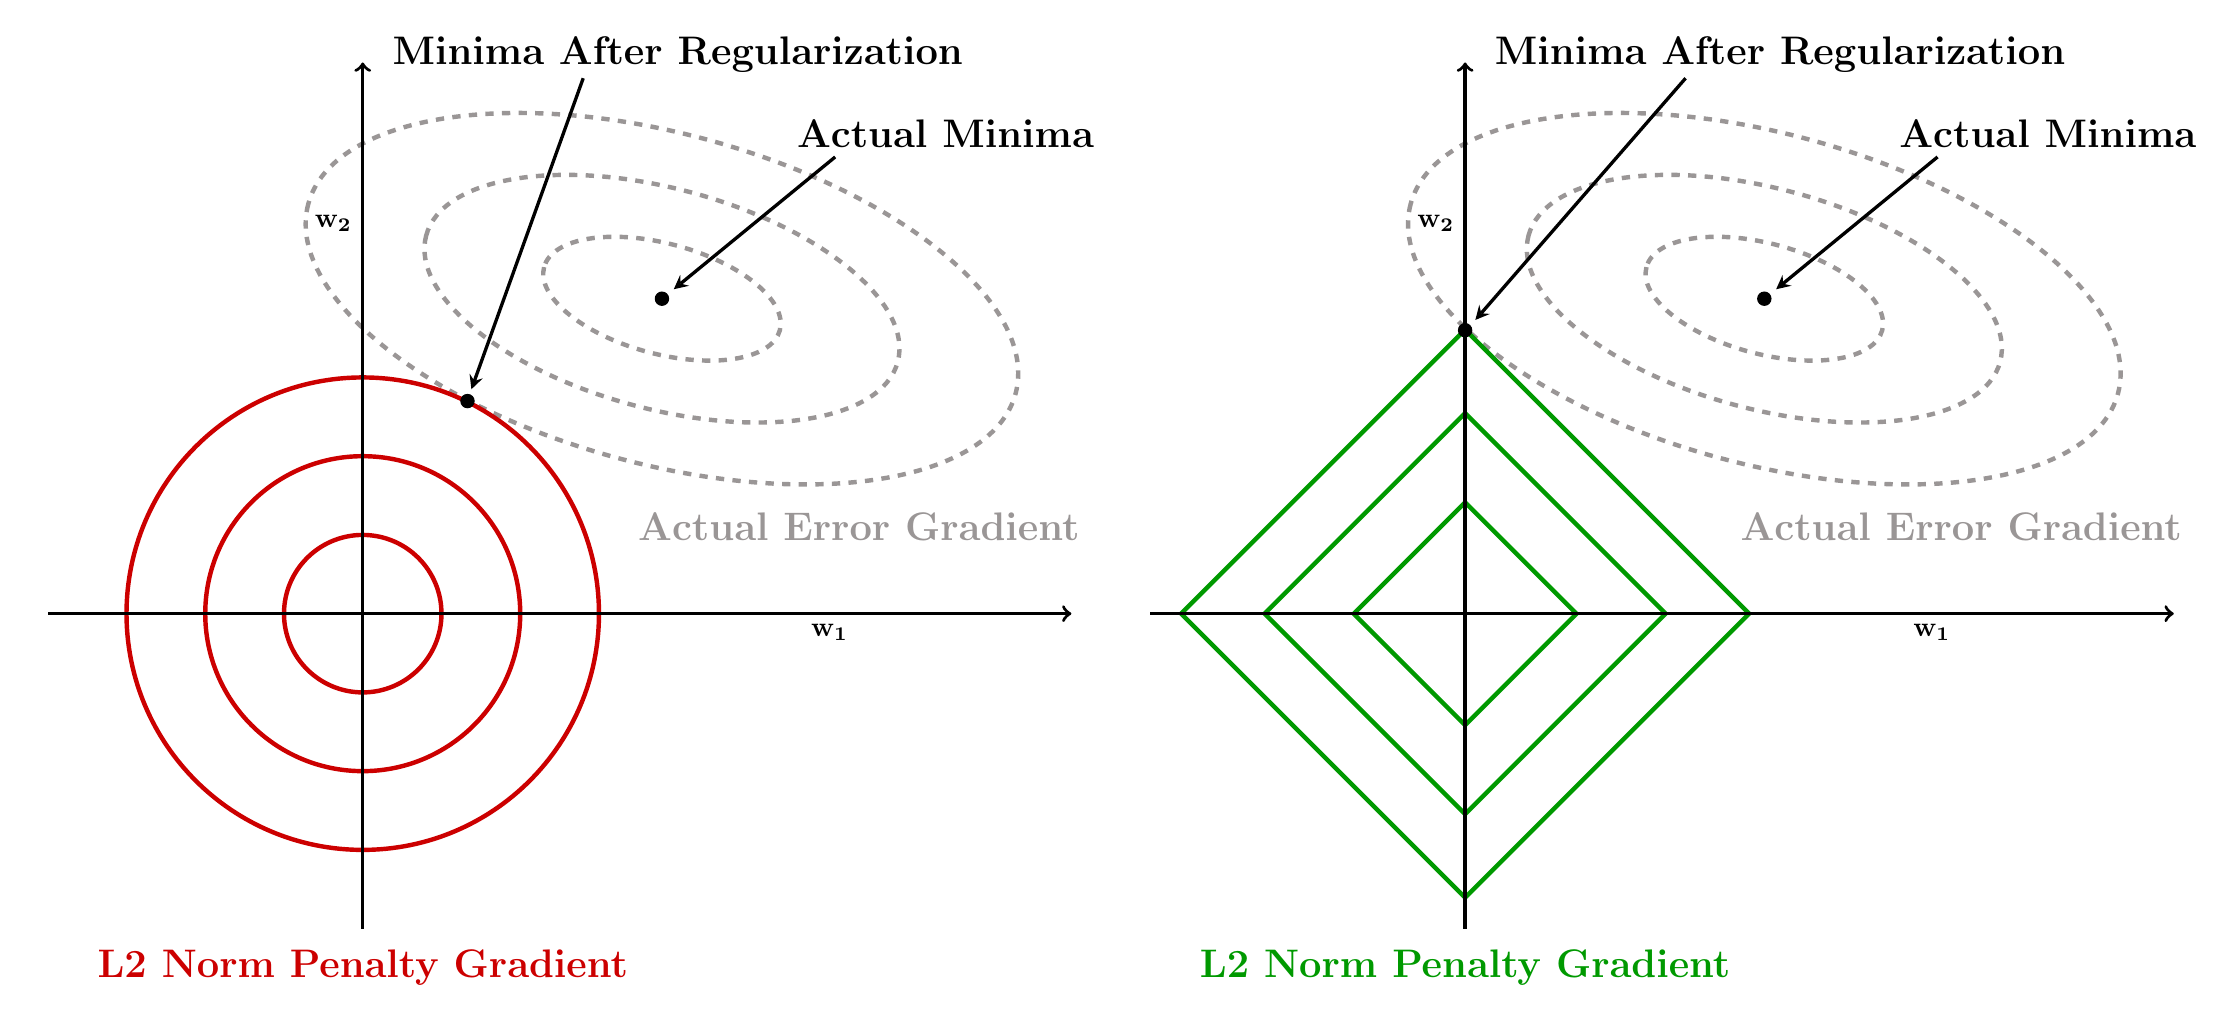
\begin{tikzpicture}

\begin{scope}[shift={(3.8,4)}]
    \foreach \r in {1,2,3}{
        \draw[ovalcolor, ultra thick, rotate=165, dashed] (0,0) ellipse ({\r*1.55} and {\r*0.7});
    }
\end{scope}

\begin{scope}[shift={(0,0)}]
    \foreach \r in {1, 2, 3}{
        \draw[myred, ultra thick, rotate=0] (0,0) circle ({\r});
    }
\end{scope}

\draw [<->, very thick] (0,7) node[below left, yshift=-1.8cm]{$\mathbf{w_2}$} |- (9,0) node[below left, xshift=-2.7cm]{$\mathbf{w_1}$}; 
\draw [-, very thick] (0,-4) node[below left]{} |- (-4,0) node[below left]{}; 

\node at (0,-4.5) {\Large\textbf{\textcolor{myred}{L2 Norm Penalty Gradient}}};
\node at (6.3,1.1) {\Large\textbf{\textcolor{ovalcolor}{Actual Error Gradient}}};


\draw[-stealth, very thick] (2.8,6.8) -- (1.38,2.85);
\filldraw (1.33,2.7) circle (2.4pt);
\node at (4,7.1) {\Large\textbf{\textcolor{black}{Minima After Regularization}}};

\draw[-stealth, very thick] (6,5.8) -- (3.95,4.12);
\filldraw (3.8,4) circle (2.4pt);
\node at (7.4,6.1) {\Large\textbf{\textcolor{black}{Actual Minima}}};

%%%%%%%%%%%%%%%%%%%%%%%%%%%%%%%%%%%%%%%%%%%%%%%%

\begin{scope}[shift={(17.8,4)}]
    \foreach \r in {1,2,3}{
        \draw[ovalcolor, ultra thick, rotate=165, dashed] (0,0) ellipse ({\r*1.55} and {\r*0.7});
    }
\end{scope}

\draw[mygreen, ultra thick, rotate around={45:(14,0)}] (13,-1) rectangle (15,1);
\draw[mygreen, ultra thick, rotate around={45:(14,0)}] (12.2,-1.8) rectangle (15.8,1.8);
\draw[mygreen, ultra thick, rotate around={45:(14,0)}] (11.45,-2.55) rectangle (16.55,2.55);

\draw [<->, very thick] (14,7) node[below left, yshift=-1.8cm]{$\mathbf{w_2}$} |- (23,0) node[below left, xshift=-2.7cm]{$\mathbf{w_1}$}; 
\draw [-, very thick] (14,-4) node[below left]{} |- (10,0) node[below left]{}; 

\node at (14,-4.5) {\Large\textbf{\textcolor{mygreen}{L2 Norm Penalty Gradient}}};
\node at (20.3,1.1) {\Large\textbf{\textcolor{ovalcolor}{Actual Error Gradient}}};


\draw[-stealth, very thick] (16.8,6.8) -- (14.13,3.73);
\filldraw (14,3.6) circle (2.4pt);
\node at (18,7.1) {\Large\textbf{\textcolor{black}{Minima After Regularization}}};

\draw[-stealth, very thick] (20,5.8) -- (17.95,4.12);
\filldraw (17.8,4) circle (2.4pt);
\node at (21.4,6.1) {\Large\textbf{\textcolor{black}{Actual Minima}}};

\end{tikzpicture}
\end{document}
